\section{The face graph of a mesh}
\begin{defi}[Undirected Graph]
    Let $\V_G$ be a set and $\E_G\subset\{e\in2^{\V_G}: |e|=2\}$ be a set of unordered pairs of elements from $\V_G$. The pair $G = (\V_G, \E_G)$ is then called undirected Graph. The elements from $\V_G$ are called vertices of $G$ and the elements from $\E_G$ are called edges of $G$.
\end{defi}
For a Graph $G=(\V_G,\E_G)$ we write
\begin{align*}
    \vcenter{\hbox{\begin{tikzpicture}
    \node (A) at (0,0) {$x$};
    \node (B) at (1,0) {$y$};
    \draw[-] (A) -- (B);\end{tikzpicture}}}
\end{align*}
if $\{x,y\}\in\E_G$. If we take all edges and points together in this way, we get the picture
of a graph with undirected edges.
\begin{ex}
    \begin{equation}\label{eq:sample_g}
    G\colon\left(\vcenter{\hbox{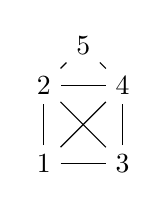
\begin{tikzpicture}[scale=0.5]
    \node (1) at (-1,-1) {$1$};
    \node (2) at (-1,1) {$2$};
    \node (3) at (1,-1) {$3$};
    \node (4) at (1,1) {$4$};
    \node (5) at (0,2) {$5$};
    \draw[-] (1) -- (2);
    \draw[-] (2) -- (3);
    \draw[-] (3) -- (4);
    \draw[-] (4) -- (2);
    \draw[-] (2) -- (5);
    \draw[-] (5) -- (4);
    \draw[-] (4) -- (1);
    \draw[-] (1) -- (3);
\end{tikzpicture}}}\right),\qquad H\colon\left(\vcenter{\hbox{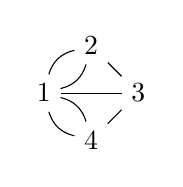
\begin{tikzpicture}[scale=0.6]
\node (1) at (-1, 0) {$1$};
\node (2) at (0, 1) {$2$};
\node (3) at (1,0) {$3$};
\node (4) at (0,-1) {$4$};
\draw[-] (1) -- (3);
\path [-] (1) edge[bend right=-30](2); 
\path [-] (1) edge[bend right=30](2); 
\path [-] (1) edge[bend right=-30](4); 
\path [-] (1) edge[bend right=30](4);
\draw[-] (3) -- (2);
\draw[-] (4) -- (3);
\end{tikzpicture}}}\right)
\end{equation}
\end{ex}
\begin{defi}[Face Graph]
    Let $M = (\mathcal{V}_M, \mathcal{F}_M)$ be a mesh and
    \begin{align*}
        \mathcal{E} = \left\{(f_1,f_2)\in\mathcal{F}_G^2: \vert f_1\cap f_2\vert =2\right\}
    \end{align*}
    The face graph of $M$ is the graph $(\mathcal{F}_M,\mathcal{E})$.
\end{defi}
\begin{ex} The face graph of the tetrahedron is given by
    \begin{equation}\label{eq:sample_g1}
    G\colon\left(\vcenter{\hbox{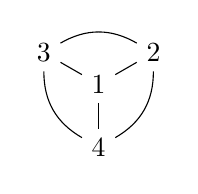
\begin{tikzpicture}[scale=0.8]
    \node (1) at (0,0) {$1$};
    \node (2) at (0.87,0.5) {$2$};
    \node (3) at (-0.87,0.5) {$3$};
    \node (4) at (0,-1) {$4$};
    \draw[-] (1) -- (2);
    \draw[-] (1) -- (3);
    \draw[-] (1) -- (4);
    \path[-] (2) edge[bend right=30] (3);
    \path[-] (3) edge[bend right=30] (4);
    \path[-] (4) edge[bend right=30] (2);
\end{tikzpicture}}}\right)
\end{equation}
\end{ex}
The face graph of a given mesh can be constructed by algorithm \ref{alg:facegraph}.
\begin{algorithm}
    \SetKwInOut{Input}{Input}
    \SetKwInOut{Output}{Output}

    \Input{A mesh $M = (\mathcal{V}_M, \mathcal{F}_M=\{f_1,f_2,f_3\ldots\})$}
    \Output{The adjacency matrix of the face graph of the mesh $M$}
    \caption{Construction of the face graph of a given mesh}
    \label{alg:facegraph}
    $G := 0\in\R^{F_M\times F_M}$\;
    \For{$i=1$ \KwTo $F_M$}
    {
        $neighbors := 0$\;
        \For{$j=1$ \KwTo $F_M$}
        {
            \If{$neighbors = 3$}{
            \textbf{break}\;
            }
            \If{$\vert f_i\cap f_j\vert = 2$ \normalfont{\textbf{and}} $i\neq j$}{
            $G_{ij} \leftarrow 1$\;
            $neighbors \leftarrow neighbors + 1$\;
            }
        }
    }
    \Return{$G$}
\end{algorithm}
Since this algorithm loops over the faces of the mesh in a nested way, the complexity of it lies in $O(F_M^2)$. As this runtime complexity has the consequence of the algorithm being very slow at execution for somewhat large meshes, the face graph is computed dynamically by \texttt{maniflow.mesh.Mesh.faceGraph}.
\subsection{A first application: \texttt{maniflow.mesh.utils.connectedComponents}}
The method \texttt{maniflow.mesh.utils.connectedComponents} decomposes the given mesh into its connected components. Now that we have an algorithm with which to compute the face graph, the connected components of a mesh can now be identified as the connected components of the face graph. These can be determined via the breadth-first traversal of the face graph. 
\begin{algorithm}
    \SetKwInOut{Input}{Input}
    \SetKwInOut{Output}{Output}

    \Input{A mesh $M = (\mathcal{V}_M, \mathcal{F}_M=\{f_1,f_2,f_3\ldots\})$}
    \Output{The connected components of the mesh $M$}
    \caption{Construction of the face graph of a given mesh}
    \label{alg:components}
    Compute the adjacency matrix $G$ using \ref{alg:facegraph}\;
    $start := 1$\;
    $n := 1$\;
    \While{$\mathcal{F}_M\neq\emptyset$}{
        Compute a breadth first traversal sequence $T_n \leftarrow \{f_{start}, f_b,f_c,\ldots\}\subseteq\mathcal{F}_M$\;
        $n \leftarrow n+1$\;
        $\mathcal{F}_M\leftarrow \mathcal{F}_M\setminus T_n$\;
        Set $1< start\leq F_M$ such that $f_{start}\in\mathcal{F}_M$\;
    }
    
    \Return{$T_1$, $T_2$, $\ldots$}
\end{algorithm}
\paragraph{Runtime analysis.} Algorithm \ref{alg:facegraph} has a runtime complexity which lies in $O(F_M^2)$. The breadth-first traversal on the face graph has a runtime\footnote{Since on a graph with the number of vertices being $V$ and the number of edges being $E$ the breadth first search has a complexity of $O(E + V)$. As every face has at most three neighbors we obtain the given runtime complexity.} complexity of $O(F_M + 3\cdot F_M) = O(F_M)$. The computation of $\mathcal{F}_M\setminus T_n$ has also quadratic complexity $O(\vert\mathcal{F}_M\vert^2)$. Thus the overall complexity of algorithm \ref{alg:components} lies in $O(F_G^2)$.
\begin{ex}
    In this example we analyse the connected components of the teapot from \texttt{examples/teapot.obj}. The teapot is displayed in figure \ref{fig:teapot}.
    \begin{figure}[h]
        \centering
        \includegraphics[scale=0.15]{img/teapot.png}
        \caption{The teapot from \texttt{examples/teapot.obj}}
        \label{fig:teapot}
    \end{figure}
    \newline\noindent The connected components can be computed using the following code
    \begin{lstlisting}
from maniflow.mesh import Mesh
from maniflow.mesh.obj import OBJFile
from maniflow.mesh.utils import connectedComponents, coincidingVertices

teapot = OBJFile.read("examples/teapot.obj")  # reading the mesh from memory
coincidingVertices(teapot)  # identifying and collapsing coinciding vertices

# now we compute the connected components
components = connectedComponents(teapot)

# we can now reconstruct meshes from these lists of faces and write them to .obj files
for i, component_list in enumerate(components):
    component = Mesh.fromFaceList(teapot, *component_list)
    OBJFile.write(component, "teapot" + str(i + 1) + ".obj")
    \end{lstlisting}
    The resulting components are shown in figure \ref{fig:teapotcomps}.
    \begin{figure}[H]
    \centering
    \subfloat[The lid of the teapot]{\includegraphics[width=0.4\textwidth]{img/teapot1.png}}\hfil
    \subfloat[The handle of the teapot]{\includegraphics[width=0.4\textwidth]{img/teapot2.png}}\hfil\\
    \subfloat[The body of the teapot]{\includegraphics[width=0.4\textwidth]{img/teapot3.png}}\hfil
    \subfloat[The spout of the teapot]{\includegraphics[width=0.4\textwidth]{img/teapot4.png}}\hfil
    \caption{The connected components of the teapot}
    \label{fig:teapotcomps}
\end{figure}
\end{ex}
\subsection{Another application: checking orientability of a \texttt{Mesh}}
Orientability is an important property of manifolds in geometry. For example, the area can only be meaningfully defined for orientable 2-manifolds. For 2-manifolds embedded in $\R^3$, orientability is equivalent to the existence of a continuous unit-normal vector field on the manifold. Similarly, we can extend the notion of orientability to meshes. If we consider a face spanned by the vertices $v_1,\ v_2$ and $v_3$, the normal vector is, for example given by\footnote{Note that $n$ does not necessarily have length $1$. But one may always obtain a unit normal vector by rescaling}
\begin{align*}
    n = (v_1 - v_2)\times (v_1 - v_3).
\end{align*}
Hence, the orientation or direction of $n$ is dependent upon the enumeration of the vertices that define the face. A priori it is not clear that two neighboring faces really do have ``compatible'' enumerations of their vertices. So it may happen that two neighboring faces have normal vectors that point in ``opposite'' directions.\footnote{An appeal to the reader's intuition. You have to be careful with these notions.}
\begin{defi}[Orientation of faces]
    Let $f = (v_1, v_2, v_3)$ be a face defined by the vertices $v_i$ for $1\leq i\leq 3$. Let $f'$ be another face that is defined by the vertices $v_1,\ v_2$ and $v_{\ast}$. We say that two faces have the same orientation, if there is a cyclic permutation $\sigma\in S_3$ such that
    \begin{align*}
        (f_1, f_2) = (f'_{\sigma(2)},f'_{\sigma(1)}).
    \end{align*}
    Where $f_i$ and $f'_i$ denote the $i$-th vertex in the faces $f$ and $f'$ respectively.
\end{defi}
In other words, two faces have the same orientation if they share an edge and that edge is traversed in opposite directions, when listing the vertices of the faces, see figure \ref{fig:orientation}.
\begin{ex}
    Consider the faces $f = (1, 2, 3)$ and $f' = (2, 3, 4)$. Then $f$ and $f'$ share the edge made up of the vertices $2$ and $3$. But both of them traverse this edge in the same direction $(2,3)$. On the other hand, if we changed the enumeration of $f'$ to $(3, 2, 4)$, the faces would have matching orientation. This is exactly the situation depicted in figure \ref{fig:orientation}.
\end{ex}
\begin{figure}[t]
    \centering
    \subfloat[Non compatible orientation]{
    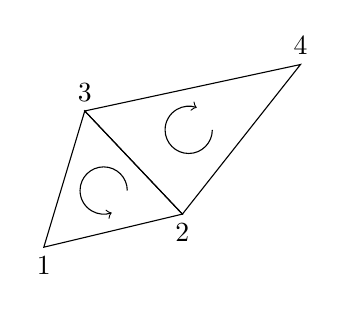
\begin{tikzpicture}
        \draw[]{} (-1.1, -1.13) -- (0.66, -0.71) node[below]{$2$} -- (-0.58, 0.6) node[above]{$3$} -- cycle node[below]{$1$};
        \draw[]{} (0.66, -0.71) -- (-0.58, 0.6) -- (2.16, 1.19) node[above]{$4$} -- cycle;
        \draw[->] (-0.04,-0.41) arc[radius=0.3cm,start angle=0,delta angle=290];
        \draw[->] (1.04,0.36) arc[radius=0.3cm,start angle=0,delta angle=-290];
    \end{tikzpicture}
    }
    \subfloat[Compatible orientation]{
    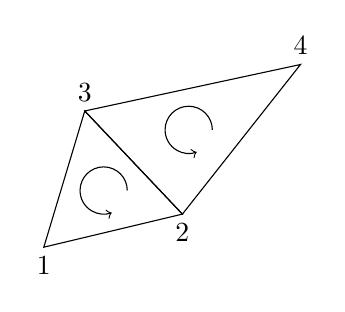
\begin{tikzpicture}
        \draw[]{} (-1.1, -1.13) -- (0.66, -0.71) node[below]{$2$} -- (-0.58, 0.6) node[above]{$3$} -- cycle node[below]{$1$};
        \draw[]{} (0.66, -0.71) -- (-0.58, 0.6) -- (2.16, 1.19) node[above]{$4$} -- cycle;
        \draw[->] (-0.04,-0.41) arc[radius=0.3cm,start angle=0,delta angle=290];
        \draw[->] (1.04,0.36) arc[radius=0.3cm,start angle=0,delta angle=290];
    \end{tikzpicture}
    }
    \caption{Two triangles with compatible and non compatible orientations}
    \label{fig:orientation}
\end{figure}
In order to determine whether a given mesh is orientable or not, we can sort of ``push'' an orientation to the mesh by traversing each of the faces in breadth-first traversal and adjusting the orientations / enumerations of vertices of each of the neighboring faces for the currently traversed face.\footnote{Of course we have to remember the faces we already considered while traversing the mesh in order to avoid faces being re-oriented twice.}
\begin{algorithm}
    \SetKwInOut{Input}{Input}
    \SetKwInOut{Output}{Output}

    \Input{A mesh $M = (\mathcal{V}_M, \mathcal{F}_M=\{f_1,f_2,f_3\ldots\})$}
    \caption{Pushing an orientation to a mesh}
    \label{alg:pushorientation}
    Store the connected components of $M$ in $\mathcal{C}$ (see algorithm \ref{alg:components})\;
    \For{$c\in\mathcal{C}$}{
    $visited := \emptyset$\;
    \For{$f\in c$}{
    \If{$f\notin visited$}{
    Store neighbouring faces to $f$ in $neighbours$\;
    \For{$f_n\in neighbours$}{
    \If{$f$ and $f_n$ do not have compatible orientations}{
    reverse the enumeration of vertices in $f_n$\;
    }
    }
    $visited \leftarrow visited \cup \{ f\}$\;
    }
    }
    }
\end{algorithm}
This is what algorithm \ref{alg:pushorientation} does. The method \texttt{maniflow.mesh.utils.pushOrientation} implements this algorithm in \maniflow{}.
Finally, to check whether a mesh is orientable or not, we only need to iterate over all surfaces in the mesh and ask whether all neighbours have a compatible orientation. This is implemented as the method \texttt{maniflow.mesh.utils.isOrientable}.
\paragraph{Runtime analysis.}  Algorithm \ref{alg:pushorientation} has a complexity of $O(F_M^2)$. % TODO: more details?
\begin{ex}[Orientability of the Moebius strip]
    Consider the \texttt{Mesh} object \texttt{moebiusMesh} from example \ref{ex:moebius_creation}. To determine whether this mesh is orientable or not, use
    \begin{lstlisting}
from maniflow.mesh.utils import isOrientable

print(isOrientable(moebiusMesh))
    \end{lstlisting}
    As expected, the output will be \texttt{False} as the Moebius strip is not orientable.
\end{ex}
\noindent Another example that is less trivial than the Moebius strip is documented in the file \href{https://gitlab.gwdg.de/yangshan.xiang/scientific-computing/-/blob/28846b92bf3f99fa84b650267886782c43791715/examples/roman_surface.ipynb}{\url{examples/roman\_surface.ipynb}} where the so-called Roman surface is discussed.
